% !Mode:: "TeX:UTF-8"
% !TeX program = lualatex

\documentclass[a4paper, 9pt, twocolumn]{extarticle}
\usepackage{polyglossia}
\usepackage{graphicx}		
\usepackage{tabularx}
\usepackage{multirow}	
\usepackage{url}
%\usepackage[ansinew]{inputenc}
\usepackage{fontspec} %LuaLaTeX
\usepackage{parskip}
\usepackage{amsmath}

\usepackage[hidelinks, unicode, english]{hyperref}

% \usepackage[]{auto-pst-pdf}
% \usepackage{pstricks}
%\usepackage{pst-plot}
% \usepackage{pst-node}
% \usepackage{multido}
% \usepackage{url}


\addtolength{\textwidth}{2.1cm}
\addtolength{\topmargin}{-2.4cm}
\addtolength{\oddsidemargin}{-1.1 cm}
\addtolength{\textheight}{4.5cm}
\setlength{\columnsep}{0.7cm}

% User defined macros
\def\x{{\mathbf x}}
\def\L{{\cal L}}
\def\SM{{\mathcal S}}
\def\SMO{{\mathcal S^{\mathrm{chroma}}}}
\def\SMS{{\mathcal S^{\mathrm{enh}}}}
\def\SMP{{\mathcal S^{\mathrm{path}}}}
\def\SMPI{{\mathcal S^{\mathrm{struct}}}}
%\def\SMPC{{\mathcal S^{\mathrm{pc}}}}
\def\SMPC{{\mathcal S^{\mathrm{pb}}}}

%added to be able to use argmax, argmin
\DeclareMathOperator*{\argmin}{arg\,min}
\DeclareMathOperator*{\argmax}{arg\,max}

\pagestyle{empty}

\begin{document}

\date{\normalsize \today}

\title{\vspace{-8mm}\textbf{\LARGE
Music Structure Analysis Summary\footnote{This is the summary for the reading assignment,
which is part of the exercise of the lecture \emph{Music Processing Analysis}, Winter Term 2015/16,
Friedrich-Alexander Universit\"at Erlangen-N\"urnberg.
Instructor: Prof.\ Dr.\ Meinard M\"uller,
Tutor: Dipl.-Ing. Stefan Baalke.
}}}

% Hier die Namen und Daten der beteiligten Autoren eintragen
\author{
{
\begin{minipage}[t]{.45\textwidth}
\center
Arnulf Becker\\
\small
Friedrich-Alexander Universit\"at Erlangen-N\"urnberg
\protect\\{} % 
\url{arnulf.becker@fau.de}
\end{minipage}%
\begin{minipage}[t]{.45\textwidth}
\center
Iñigo Fern\' andez\\
\small
Friedrich-Alexander Universit\"at Erlangen-N\"urnberg
\protect\\{} % 
\url{inigo.fernandez@fau.de}
\end{minipage}%
}
}
 
\maketitle
\thispagestyle{empty}


%%%%%%%%%%%%%%%%%%%%%%%%%%%%%%%%%%%%%%%%%%%%%%%%%%%%%%%%%%%%%%%%%%%%%%%%%%%%%%
\section{General Principles} 
\label{section:generalPrinciples}
%Alternative names: intro, basics...
%%%%%%%%%%%%%%%%%%%%%%%%%%%%%%%%%%%%%%%%%%%%%%%%%%%%%%%%%%%%%%%%%%%%%%%%%%%%%%

\subsection{Musical Structure}  
% Mixture of sections 'intro' and 4.1.2 from the book
The sounds that conform music are not organized in a random way: they are combined conforming musical structures such as phrases, motifs or sections. Those structures are again combined and form higher-level sections that determine the overall layout of the composition, also called \textbf{musical structure}. The names of the mentioned high-level sections may vary depending on the kind of music we are analysing, as well as the way they are arranged. 

\medskip

In Western music, the musical structure often follows certain patterns. The simplest one is the \textbf{strophic form}, which consists of a sequence of a repeated part resulting in a $A_{1}A_{2}A_{3}A_{4}...$ structure, usually used in folk song or nursery rhymes. Medleys or potpourris (concatenation of popular songs) use the so called \textbf{chain form}, a sequence of unrelated parts ($ABCD...$), sometimes with repeats ($A_{1}A_{2}B_{1}B_{2}C_{1}C_{2}...$). Another form is the \textbf{rondo form}, where a recurring theme alternates with contrasting sections $A_{1}BA_{2}CA_{3}DA_{4}...$

\medskip

In Western classical music, one of the most important musical structures is the \textbf{sonata form}. It consists of an \textbf{exposition} ($E$), a \textbf{development} ($D$), and a \textbf{recapitulation} ($R$), where the exposition is repeated once. At a coarse level, that recapitulation can be regarded as a repetition of the exposition, although at a finer level they are different. Sometimes, one can find an additional \textbf{introduction} ($I$) and a closing \textbf{coda} ($C$), thus yielding the form $ IE_{1} E_{2} DRC $. 

\medskip

In popular music, the most typical parts are the \textbf{verse} ($V$ ) and the \textbf{chorus} ($C$)
sections. Each verse usually employs the same melody (possibly with slight modifications), while the lyrics change for each verse. The \textbf{chorus} or \textbf{refrain} typically consists of a melodic and lyrical phrase which is repeated. Sometimes, pop songs may start with an \textbf{intro} ($I$) and close with an \textbf{outro} ($O$). Finally, verse and chorus sections may be connected by an additional part called a \textbf{bridge} ($B$). The verse and chorus are usually repeated throughout a song, while the intro and the outro appear only once. Some pop songs may also have a \textbf{solo} where an instrument plays a melody. 


\subsection{Segmentation and Structure Analysis}

%%%%%%%%%%%%%%%%%%%%%%%%%%%%%%%%%%%%%%%%%%%%%%%%%%%%%%%%%%%%%%%%%%%%%%%%%%%%%%
%from book 4.1.1

The main goal of \textbf{structure analysis} is to find and understand the relationships between the sections of the musical structure. \textbf{Repetitions} play an important role in music, where rhythms, harmonies or melodies are often repeated. On the other hand, \textbf{contrast} is the difference between successive sections of different character regarding tempo, loudness or instrumentation. A further principle is that of \textbf{variation}, where motifs and parts are picked up again in a transformed form. Finally, a section is often characterized by some sort of \textbf{homogeneity}, being the all its features according to some criteria. All of those principles have to be considered with time in mind: music happens in \textbf{time} (opposed to paintings for example) and the order of events is essential in the analysis. 


%For example, some of them may be repeated with slight changes, as in the case of a pop song, that normally has several similar \textit{verses}. Those verse sections may vary in instrumentation, tempo, lyrics, melody and many other aspects. If they do, that section is called a \textbf{variation}. The task of the analysis is to identify them as similar and to correctly group them in the same musical category \textit{verse}. % 
%%\textbf{Repetitions} are one of the phenomena that happen in a piece of music. Variations are similar
%
% as well as to analyse the progression of the different musical categories. Repetitions are one of the phenomena studied by musical structure analysis, 

The first step for analysing the relation of the segments is to identify them. In a more general context, \textbf{segmentation} refers to partitioning a document into multiple parts that are easier to analyse than the original document. In music, segmentation decomposes an audio stream into acoustically meaningful sections. At a fine level, it may aim to find the boundaries between individual notes or beat positions. At a coarser level, the goal may be to de detect changes in instrumentation or harmony to find the boundaries between \textit{verse} and \textit{chorus} sections. Also, discriminating between silence, speech, and music, finding the actual beginning of a music recording or separating the applause at the end of a performance are typical segmentation tasks.

The first step in segmentation of music is to transform the given audio into a suitable feature representation. As discussed in previous chapters, there is various alternatives to choose depending on the focus of the study. 

When focusing in harmony and melody, \textbf{chroma features} are one of the most typical features. The drawback of using them is that we lose some information about pitches that could be useful for humans to distinguish the timbre, and so the instrumentation. However, in structure analysis is unnecessary to be so precise. Instead, mid-level representations correlated to instrumentation and timbre are enough. The \textbf{mel-frequency cepstral coefficients} (MFCCs) are often used, though they were originally developed for speech recognition.

Tempo and beat information can also be used in homogeneity-based approaches. Instead of extracting such information explicitly, a mid-level feature representation correlated to tempo and rhythm, a \textbf{tempogram} suffices.

Of course, one may use various of the methods mentioned before to do different analysis and get to a better understanding of the musical structure.

%%%%%%%%%%%%%%%%%%%%%%%%%%%%%%%%%%%%%%%%%%%%%%%%%%%%%%%%%%%%%%%%%%%%%%%%%%%%%%
\section{Mathematical tools: Self Similarity Matrix}
\label{section:ssm}
%from book 4.2
%%%%%%%%%%%%%%%%%%%%%%%%%%%%%%%%%%%%%%%%%%%%%%%%%%%%%%%%%%%%%%%%%%%%%%%%%%%%%%
\subsection{Basic Definitions and Principles}
\label{subsection:ssmBasic}

To study musical structures and their mutual relations, we convert the music signal into a feature sequence and then compare each element of the sequence with all other elements. This results in a \textbf{self-similarity matrix} (SSM), whose elements $s(x,y)$ are high in case the elements $x,y$ are similar and small otherwise. The comparison of the $N$ features with each other results in a $N$-square \textbf{self-similarity matrix S} defined by $\textbf{S}(n,m):=s(x_{n}, x_{m})$. The tuple ($n,m$) is called a \textbf{cell} of \textbf{S}, and the value \textbf{S}($n,m$) is the \textbf{score} of the cell ($n,m$).

Obviously the concept of self-similarity matrices is closely related to the concept of cost matrices. However, instead of a cost measure $c$ we now use a similarity measure $s$. And
instead of comparing two sequences $X$ and $Y$ with each other, we now compare a single sequence $X$ with itself.

A common \textbf{similarity measure} $s$ is the absolute value of the inner product, $s(x,y):=|\langle x,y \rangle|$, but of course there are many more possibilities. Their suitability depends on the properties of the considered features and vice versa. It is also common to normalize the similarity measure so it has a value between $[0,1]$. 

In this case, the SSM has a diagonal with large values, because $s(x_{n},x_{n})=1$ for all $n$. Recurring patterns become visible in the SSM in the form of structures. The most commons ones are \textbf{block}-like structures (corresponding to musical properties that remain constant through time, and so related to homogeneity), and \textbf{paths} parallel to the main diagonal that appear when  sequences are repeated. Those paths may not be perfectly parallel to the main diagonal, due to relative tempo differences between the two related segments.

(image of SSMs)

(examples of sssm interpretations) page 183 of the book

To formalize paths and block structures, some other basics have to be defined first. \autoref{fig:ssmPathBlock} shows a graphical description of them. A segment is a set $\alpha=[s:t]$ of features specified by the index $s$ of the starting feature and the index $t$ of its last feature. We will use $|\alpha|:=t-s+1$ to denote the length of $\alpha$. A \textbf{path} over $\alpha$ of length $L$ is a sequence $P=((n_{1},m_{1}), (n_{2},m_{2}), ..., (n_{L},m_{L})$ of cells $(n_{l}, m_{l})$ that satisfy the boundary condition $m_{1}=s$ and $m_{L}=t$ and the step size condition $(n_{L+1},m_{L+1})-(n_{L},m_{L})\in \Sigma$, where $\Sigma$ denotes the admissible set size. As in the warping path case, we normally use $\Sigma=\{(2,1), (1,2), (1,1)\}$.

Every path $P$ has two two segments $\pi_{1}:=[n_{l}:n_{L}$ and $\pi_{1}:=[m_{l}:m_{L}]$ associated, defined by its projections. Logically, $\pi_{2}(P)= \alpha$. The other segment $\pi _{1} (P)= \alpha$ is called the \textbf{induced segment}. The \textbf{score} $\sigma (P)$ of $P$ is defined as\[\sigma(P):= 	\sum_{l=1}^{L}\textbf{S}(n_{l}, m_{l})\]

Note that each path over the segment \alpha encodes a relation between \alpha and an induced segment, where the score $\sigma(P)$ yields a quality measure for this relation.

%-----------------------
\begin{figure}[h]
\centering
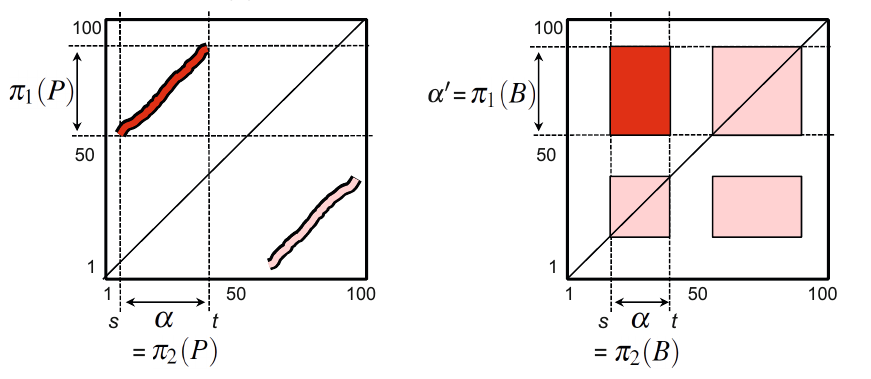
\includegraphics[width=\linewidth]{images/SSMpathBlocks.png}
\caption{SSM with path and block structures.}
\label{fig:ssmPathBlock}
\end{figure}
%-----------------------

A \textbf{block} over a segment  $\alpha=[s:t]$ is a subset $B=\alpha' \times \alpha$ for some segment $\alpha'=[s':t']$. As for paths, we define the two projections $\pi_{1}(B)= \alpha'$ and $\pi_{2}(B)= \alpha$, and call $\alpha'$ the \textbf{induced segment}. The score of the block is given by \[\sum_{(n,m)\in B}^{L}\textbf{S}(n, m)\].
In case the  measure $s$ is symmetric, the self-similarity matrix and the similarity relations between segments are symmetric as well. Normally, if a segment $\alpha_{1}$ is similar to $\alpha_{2}$ and $\alpha_{2}$ is similar to $\alpha_{3}$, $\alpha_{3}$ should be similar to $\alpha_{1}$. This is called \textbf{transitivity}, and happens if the similarity measure also has that property. Consequently, paths and blocks often appeare in groups that fulfill certain symmetry and transitivity properties. For example, if there is a block $B=\alpha'\times\alpha$, then there is also a block $\alpha\times\alpha'$. This leads to additional blocks $\alpha'\times\alpha'$ and $\alpha\times\alpha$. 

Most computational approaches to music structure follow these steps:

\begin{enumerate}
\item Music is transformed into a feature sequence.\item A self-similarity matrix is computed based on a similarity measure.\item Blocks and paths are detected.\item Similar segments are grouped applying a clustering step.
\end{enumerate}


\subsection{Enhancement Strategies}
\label{subsection:ssmEnhancement}

Computerized music structure analysis is an error-prone and fragile task, as both the grouping and the block and path extraction step are deteriorated because of the musical variations. However, there are some strategies for enhancing the properties of SSMs to make the process more reliable. 

\subsubsection{Feature Preprocessing}
\label{subsubsection:ssmEnhancementFeaturePreprocessing}

Considering a modified chroma representation may result in a SSM with more recognizable patterns. This task is better explained in another chapter, but in broad terms it is based on two parameters: The length parameter $l$, to average the feature values over $l$ consecutive frames, and the downsampling parameter $d$ which reduces the feature rate. The effects can be seen in the \autoref{fig:ssmDownsampling}:


%-----------------------
\begin{figure}[h!]
	\centering
	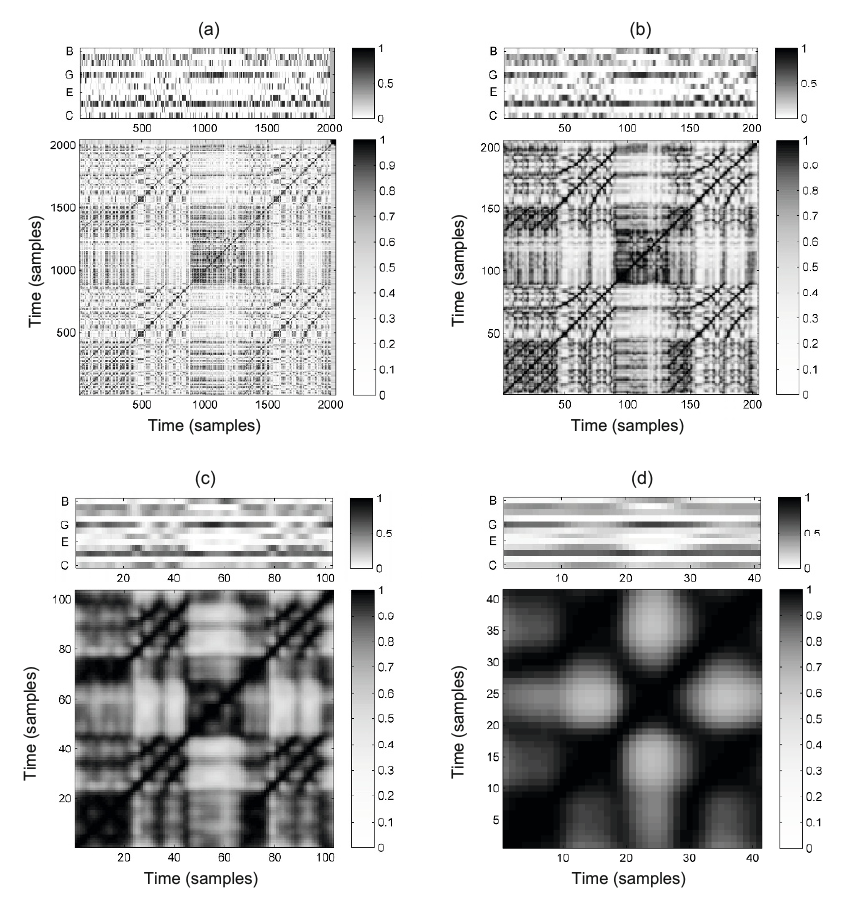
\includegraphics[width=\linewidth]{images/ssmDownsampling.png}
	\caption{(a) Usage of original normalized chroma features (10 Hz). (b) Applying $l$=40 and $d$=10 (1 Hz). (c) Applying $l$= 160 and $d$=20 (0.5 Hz). (d) Applying $l$=480 and $d$=50 (0.2 Hz).}
	 \label{fig:ssmDownsampling}
\end{figure}
%-----------------------


Many of the details have been smoothed out, and some
of the structurally relevant path and block structures have become more prominent. Moreover,reducing the feature rate improves the computational efficiency for subsequent processing steps. Further increasing the smoothing length and reducing the feature rate results in an enhancement of block-like structures. However, using large smoothing windows relevant path structures may be lost. A good strategy for adjusting and reducing the feature rate is based on \textbf{adaptive windowing}, where the analysis windows are determined by previously extracted onset
and beat positions. 


\subsubsection{Path smoothing}
\label{subsubsection:ssmEnhancementPathSmoothing}


Paths that run parallel to the main diagonal are important structural elements of similarity matrices, but the automated detection of them constitutes a difficult problem due to distortions. 

To some extent, structural properties of the SSM may be augmented by using longer analysis windows in the feature computation step. This, however, may also smooth out important details. An alternative is to apply image processing techniques. Relevant paths run along the direction of the main diagonal. To augment such paths, one can apply an averaging filter (or low-pass filter) in the direction of the main diagonal, which results in an emphasis of diagonal structures and a softening of others, nondiagonal ones.

We can obtain a smoothed similarity matrix $\textbf{S}_{L}$ from a $N \times N$  SSM applying the following formula: 
\[\textbf{S}_{L}(n,m):= \frac{1}{L}\sum_{l=0}^{L-1}\textbf{S}(n+l,m+l)\]
In other words, the value $\textbf{S}_{L}(n,m)$ is obtained by averaging the values of the diagonal of length $L$ starting at position $(n,m)$. Where the matrix $\textbf{S}$ is not defined, we extend it by zero-padding. 

A simple filtering along the main diagonal only works well if there are no relative tempo differences between the segments. However, this is violated when a part is repeated with a faster or slower tempo. This results in a path that does not run exactly parallel to the main diagonal (in particular at the beginning), so that applying an averaging filter in the direction of the main diagonal destroys some of the path. To deal with such relative tempo differences, one idea is to apply a \textbf{multiple filtering} approach, where the SSM is smoothed along various directions similar to the direction of the main diagonal. Each such direction corresponds to a tempo difference and results in a separate filtered matrix. The final self-similarity matrix is obtained by taking the cell-wise maximum over all these matrices.  

%-----------------------
\begin{figure}[h]
\centering
  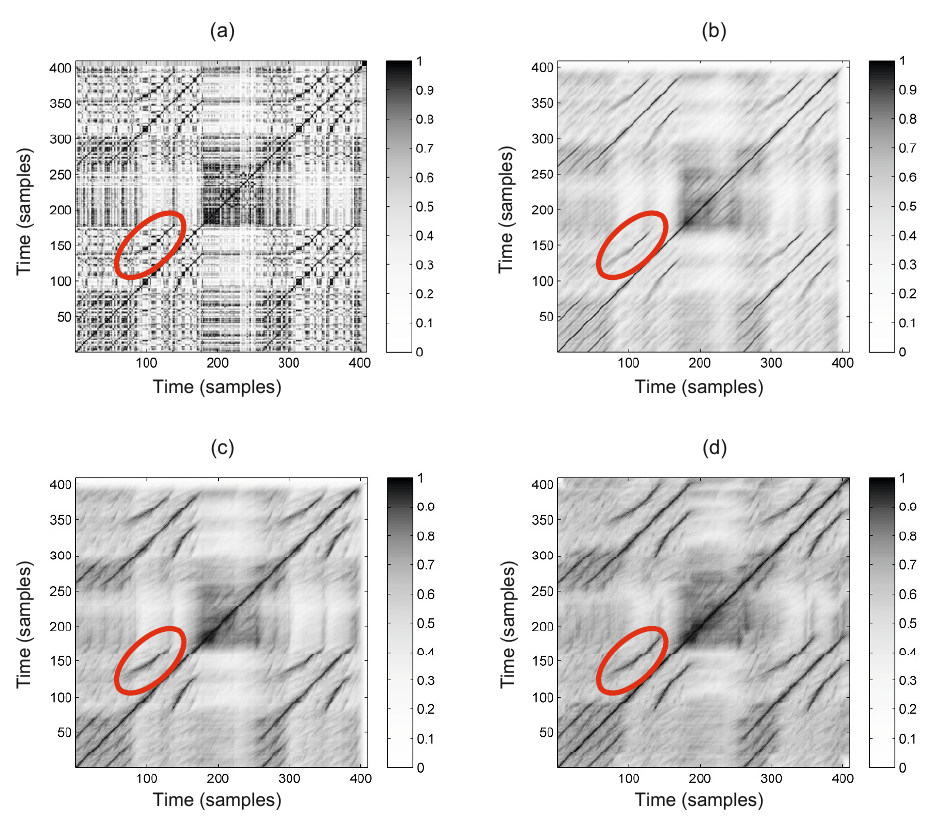
\includegraphics[width=\linewidth]{images/ssmPathSmoothing.png}
\caption{(a) Original SSM using chroma features (resolution of 2 Hz). (b) SSM after applying diagonal smoothing. (c) SSM after applying tempo-invariant smoothing. (d) SSM after applying forward–backward smoothing.}
\label{fig:ssmPathSmoothing}
\end{figure}
%-----------------------

This is easier to see with an example. Assume we have  two repeating segments $\alpha_{1}$ and $\alpha_{2}$ played at the same tempo. The direction of the resulting path is (1, 1). Next, assume the second segment $\alpha_{2}$ is played at half the tempo. Then the direction of the path is (1, 2). If the tempo difference between two segments is given by a real number  \theta (the second segment played \theta times slower than the first one), the resulting gradient is $(1,\theta)$. We define the self- similarity matrix smoothed in the direction of (1, \theta) by
\[\textbf{S}_{L,\theta}(n,m):=\frac{1}{L}\sum_{l=0}^{L-1}\textbf{S}(n+l,m+[l·\theta])\]
where $[l·\theta]$ denotes the integer closest to $l·\theta$. Again, we must apply zero-padding to the matrix $\textbf{S}$ so that $\textbf{S}_{L,\theta}$ is defined for every $n,m$.

In practice, one does not know the tempo difference that may occur.  Also, the relative tempo difference may change over time. The idea is to consider a (finite) set \Theta  consisting of various tempo parameters \theta. We compute a matrix $\textbf{S}_{L,\theta}$ for each \theta, and obtain a final matrix $\textbf{S}_{L,\Theta}$ by a cell-wise maximization over all \theta: 
\[\textbf{S}_{L,\theta}(n,m):=\max_{\theta\in\Theta}\textbf{S}_{L,\theta}(n,m)\]

In practice, one can use prior information about tempo differences to determine the set \Theta. It rarely happens that the relative tempo difference is larger than 50 percent, so \Theta can be chosen from −50 to +50 percent. Further-
more, the tempo range can be covered well by considering only a small number of tempo parameters. A typical choice could be  $\Theta=\{0.66, 0.81, 1.00, 1.22, 1.50\}$.
This smoothing works in the forward direction. Better results can be achieved if additionally applying the filter in a backward direction. The final self-similarity matrix is obtained taking the cell-wise maximum over the forward- and backward-smoothed matrices. 


\subsubsection{Transposition Invariance}
\label{subsubsection:ssmEnhancementTransInvariance}

Often, certain musical parts are repeated in a transposed form, where the melody is moved up or down in pitch by a constant interval. However, because of those transpositions, the relation between sections is not reflected in the SSM. We can make the SSM reflect them even in the presence of key transpositions by calculating the $i$-\textbf{transposed self-similarity matrix} $\rho^i(\textbf{S})$ defined by

%formulaca
\[\rho^i(\textbf{S})(n,m):=s(\rho^{i}(x_{n}), x_{m})\]

where \rho  is the cyclic shift operator we defined for the chroma features. Obviously, $\rho^{12}(\textbf{S})=\textbf{S}$. Intuitively, $\rho^i(\textbf{S})$ describes the similarity between the original music  and the music transposed by $i$ semitones upwards.

Taking a cell-wise maximum over the twelve different cyclic shifts, we obtain a \textbf{transposition-invariant self-similarity matrix}  defined by $\textbf{S}^{TI}$ defined by
\[\textbf{S}^{TI}(n,m):=\max_{i\in[0:11]}\rho^i(\textbf{S})(n,m)\]
We store the maximizing shift indices in an additional $N$-square matrix $\textbf{I}$, the \textbf{transposition index matrix:}
\[\textbf{I}(n,m):=\argmax_{i\in[0:11]}\rho^i(\textbf{S})(n,m)\]

%-----------------------
 \begin{figure}[h]
 \centering
 	\includegraphics[width=\linewidth]%5cm
 		{images/transpositionMatrix.png}
 	\caption{Variants of SSMs for the song “In the year 2525” by Zager and Evans. (a) Original
SSM using chroma features.(b) Path-enhanced SSM. (c) 1-transposed SSM.(d) 2-transposed SSM.(e) Transposition-invariant SSM.(f) Transposition index matrix.}
 \label{figure:transpInxexMatrix}
 \end{figure}
%-----------------------

The transposition index matrix values are usually coded with colours, as shown in \autoref{figure:transpInxexMatrix}.

The value $i=0$ for a cell $(n, m)$ indicates that the chroma vector $x_{m}$ is closer to $x_{n}$ than any shifted version of $x_{n}$. Note, however, that this does not necessarily mean that $x_{m}$ is close to $x_{n}$ in absolute terms. At all positions where the conventional self-similarity matrix reveals paths of low cost, $i$ will take the value $i=0$. The value $i=1$ for a cell $(n, m)$ indicates that $x_{n}$  becomes most similar to $x_{m}$ when shifted one semitone upwards, and so on for other values of $i$. 

Introducing transposition invariance may increase the noise, and therefore, the transposition-invariant matrix should be computed on the basis of smoothed matrices. 


\subsubsection{Thresholding}
\label{subsubsection:ssmEnhancementThresholding}

In many music analysis applications, self-similarity matrices are further processed by suppressing values that fall below a given threshold. On the one hand, this leads to reduction of unwanted noise, leaving only significant structures. On the other hand, weaker but still relevant information may be lost. The thresholding strategy has to be carefully chosen. 

The simplest strategy is to apply \textbf{global thresholding}, where all values below a given threshold parameter $\tau>0$ are set to zero:

\[\textbf{S}_{\tau}(n,m):= 
 \begin{cases} 
      \textbf{S}(n,m) & if  \textbf{S}_{\tau}(n,m)\geq\tau \\
      0 & otherwise 
   \end{cases}
\]  

Also, we may also apply \textbf{binarization} by setting all values above the threshold to one and all others to zero. Instead of binarization, one may perform a \textbf{scaling} where the range $[\tau, \nu]$ is linearly scaled to $[0, 1]$.  Sometimes it may be beneficial to introduce an additional \textbf{penalty} parameter $\delta\leq0$, setting all original values below the threshold to the value $\delta$.

%-----------------------
 \begin{figure}[h]
 \centering
 	\includegraphics[width=\linewidth]%5cm
 		{images/ssmThreshold.png}
 	\caption{(a) SSM from \autoref{fig:ssmPathSmoothing}. (b) SSM after thresholding and
 	binarization $(\tau=0.75)$. (c) SSM after thresholding and scaling $(\rho=0.2)$. (d) SSM after thresholding and scaling $(\rho=0.05)$.
}
 \label{figure:ssmThreshold}
 \end{figure}
%-----------------------


The threshold $\tau$  can also be chosen in a \textbf{relative} way by keeping \rho·100\% of the cells with the highest values, where  $\rho\in[0,1]$ is the relative threshold parameter.  Thresholding can also be performed using a \textbf{local} strategy in a column- and row-wise fashion. To this end, for each cell $(n, m)$, the value $\textbf{S}(n, m)$ is kept if it is among the \rho·100\% of the largest cells in row $n$ and at the same time among the \rho·100\% of the largest cells in column $m$, all other values being set to zero. The suitability of a thresholding setting depends on the application. Often, suitable thresholds are learned and optimized using supervised learning procedures.

%-----------------------
 \begin{figure}[h]
 \centering
 	\includegraphics[width=\linewidth]%5cm
 		{images/ssmProcessed.png}
 	\caption{(a) Original SSM using chroma features. (b) SSM after diagonal smoothing. (c) SSM after tempo-invariant and forward–backward smoothing. (d) Transposition-invariant SSM.
(e) Transposition index matrix. (f) SSM after thresholding with penalty and scaling $(\rho=0.2, \delta=−2)$.}
 \label{figure:ssmProcessed}
 \end{figure}
%-----------------------


%%%%%%%%%%%%%%%%%%%%%%%%%%%%%%%%%%%%%%%%%%%%%%%%%%%%%%%%%%%%%%%%%%%%%%%%%%%%%%
\section{Repetition based Segmentation and Audio Thumbnailing}
\label{section:repetition}
%%%%%%%%%%%%%%%%%%%%%%%%%%%%%%%%%%%%%%%%%%%%%%%%%%%%%%%%%%%%%%%%%%%%%%%%%%%%%%

The main goal of \textbf{audio thumbnailing} is to automatically determine the most representative
section of a audio recording. In many cases the chorus or the main theme are good candidates for
this. 
In order to find this section a \textbf{fitness measure} is used to rate every part. It describes
both how well it is suited to explain other elements and how much of the whole music recording these
related segments cover. The audio thumbnail is then the segment of maximum fitness.


%-----------------------
\begin{figure}[h]
\centering
  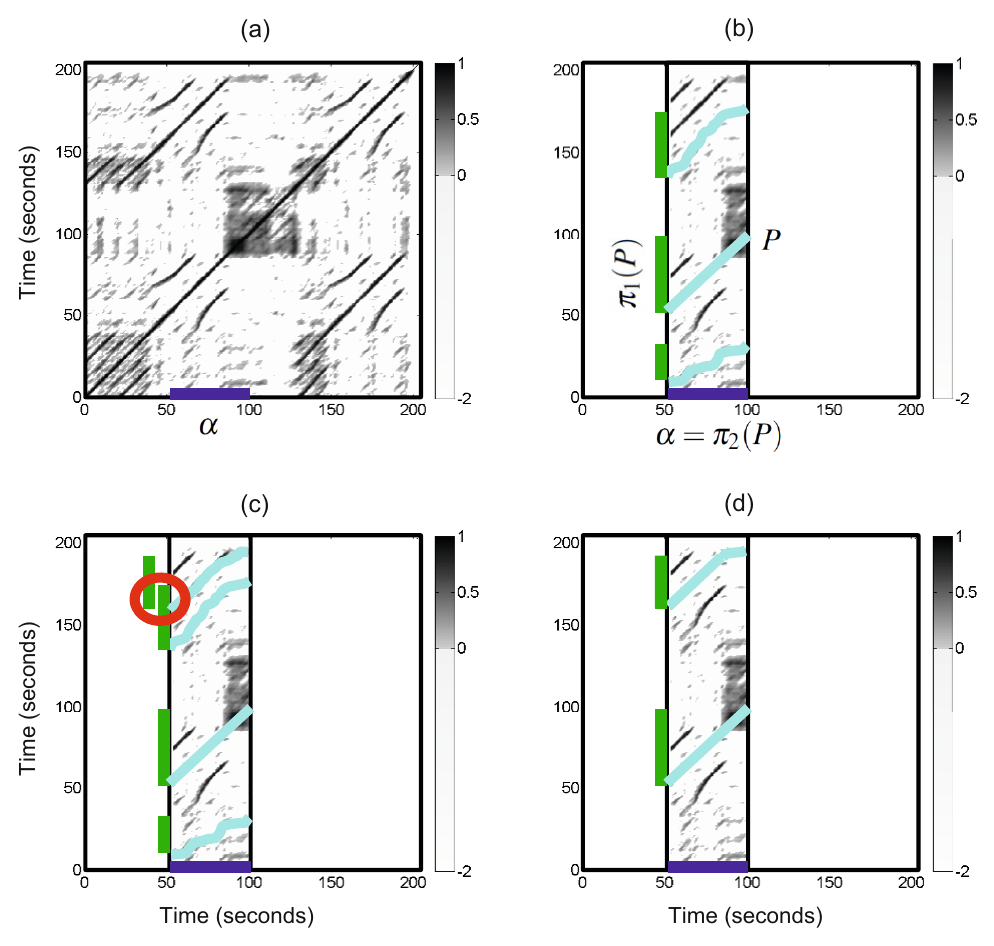
\includegraphics[width=\linewidth]{images/pathFamilies.png}
	\caption{SSM with various paths over the segment $\alpha=[50:100]$. The induced segments are indicated on the vertical axis. (a) SSM. (b) Paths forming a path family. (c) Paths not forming a path family (induced segments overlap). (d) Paths forming an optimal path family.}
	\label{fig:pathFamilies}
\end{figure}
%-----------------------

\subsection{Scape Plot Representation}
\label{subsection:scapePlot}

A scape plot is a method to visualize the fitness value of each possible segment. As can be seen in 
\autoref{fig:scapePlot} on the y-axis there is segment length and on the x-axis the center of the
respective segment. It has a triangle shape because a segment covering the whole music recording only has one center point, whereas a segement with length one can have its center on all positions.
The third axis, which represents the fitness value, is visualized by a color gradient within the
triangle.

%-----------------------
\begin{figure}[h]
	\centering
	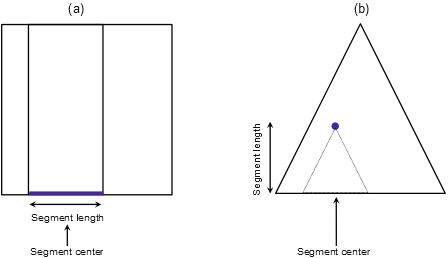
\includegraphics[width=\linewidth]{images/scapePlot.png}
	\caption{Definition of scape plot representation. (a) Schematic SSM with segment. (b) Schematic
scape plot with segment.}
	\label{fig:scapePlot}
\end{figure}
%-----------------------

%%%%%%%%%%%%%%%%%%%%%%%%%%%%%%%%%%%%%%%%%%%%%%%%%%%%%%%%%%%%%%%%%%%%%%%%%%%%%%
\section{Novelty based Segmentation}
\label{section:novelty}
%%%%%%%%%%%%%%%%%%%%%%%%%%%%%%%%%%%%%%%%%%%%%%%%%%%%%%%%%%%%%%%%%%%%%%%%%%%%%%

The objective of novelty-based structure analysis is to locate points where musical changes occur, thus marking the transition between two subsequent structural parts. There are various approaches for doing so, two of them will be covered. 

\subsection{Novelty function and Checkerboard  Kernel}
\label{subsection:noveltyKernel}

In music it is quite common to find a homogeneous segment followed by another homogeneous segment in
contrast with the previous one (a section played by strings and one played by brass for example). In that case, SSMs reveal block-like structures. The goal of novelty detection is to identify the boundary between those sections. This is achieved analysing the \textbf{novelty function}, obtained  by correlating a checkerboard-like kernel along the main diagonal of the SSM. The peaks in this function indicate where changes happen in the audio signal. For example, using MFCCs, these peaks are good indicators for changes in timbre or instrumentation.

Let's consider an audio with two homogeneous but contrasting sections. The SSM will have dark blocks on the main diagonal  corresponding to high similarity of the sequences with themselves. In contrast, light regions outside these blocks express that there is a low cross-similarity between the sections. Thus, to find the boundary between the two sections one needs to identify the crux of the ckeckerboard.

To do so we can correlate the SSM with a kernel that looks like a checkerboard. The simplest one is the 

%%
%% 2x2 K kernel
%%

This kernel can be expressed as the difference between two kernels, as shown in the formula. The first kernel measures self-similarity, and its value is high when the two regions are homogeneous. The second kernel measures cross-similarity, and its value is high when the two regions are similar to each other. The difference of those two values estimates the \textbf{novelty}, which is high when two regions are self-similar but different from each other. 

%-----------------------
 \begin{figure}[h]
 \centering
 	\includegraphics[width=\linewidth]%5cm
 		{images/checkerboardKernel.png}
 	\caption{Checkerboard kernel functions of size $M=21 (L=10)$. (a,b) Box-like checkerboard kernel and 3D plot. (c,d) Gaussian checkerboard kernel and 3D plot.}
 \label{figure:checkerboardKernel.png}
 \end{figure}
%-----------------------


Normally the kernels used are larger, as we are interested in changes on a larger time scale. To obtain those kernels, we define a size of the kernel $M$ given by $M=2L+1$. The box-kernel of size $M$ is an $M\times M$ square matrix whose indexes go from $[-L,L]$, and defined by $\textbf{K}=sgn(k)·sgn(l)$ where $k,l\in[-L,L]$ and "sgn" is the sign function (being -1 for negative numbers, 0 for zero and 1 for positive numbers). For example, for $L=2$ one obtains the following kernel:

%%
%%  bigger kernel palette
%%

This box-kernel can also be smoothed by point wise multiplying it with a Gaussian function defined by  $\phi(s,t):=exp(-\epsilon^2(s^2+t^2))$ thus obtaining

\[\textbf{K}_{Gauss}(k,l)=\phi(k,l)·\textbf{K}_{Box}(k,l)\]

The normalization of the kernel is also very important, specially when combining and fusing information obtained from kernels of different size, and can be performed as follows

\[\textbf{K}_{Norm}(k,l)=\frac{\textbf{K}_{Gauss}(k,l)}{\sum_{kxl\in[-L:L]}|\textbf{K}_{Gauss}(k,l)|}\]


To detect the corner points we slide the kernel $\textbf{K}$ along the main diagonal of the SSM and sum up the element-wise product, getting a $\Delta_{Kernel}(n)$ \textbf{novelty function}:

\[\Delta_{Kernel}(n):=\sum_{kxl\in[-L:L]}\textbf{K}(k,l)\textbf{S}(n+k, n+l)\]

When the kernel is positioned in a uniform region, the positive and negative values sum up to zero and $\Delta_{Kernel}(n)$ becomes small. When the kernel is at the crux, the values sum up to a large value $\Delta_{Kernel}(n)$. 

%-----------------------
 \begin{figure}[h]
 \begin{center}
 	\includegraphics[width=\linewidth]%5cm
 		{images/kernelSizes.png}
 	\caption{(a) SSM using tempo-based features. (b–d) Novelty functions derived from (a) using a kernel of small/medium/large size. (e) SSM from Figure 4.7b using chroma-based features. (f–h) Novelty functions derived from (e) using a kernel of small/medium/large size.}
 \end{center}
 \label{figure:kernelSizes.png}
 \end{figure}
%-----------------------


The size of the kernel has a significant impact on the novelty function. Smaller kernels are used for detecting novelty on a short time scale, whereas large kernels are suited for detecting boundaries in a coarse level. A small kernel can lead to a noisy novelty function with many peaks, particularly when SSM contains path structures. Using a larger kernel results in a smoother novelty function. A similar effect is achieved by smoothing the SSM, because that often leads to an enhancement of the blocks. 

Peak selection strategy is also a delicate step that influences on the final result. Adaptive thresholding techniques may be applied to the novelty function so that a peak is only selected when its value exceeds the local average. We can also impose a minimal distance between subsequent peaks to reduce wrong boundary detections.

% \subsection{Structure Features}
% \label{subsection:structureFeatures}



%%%%%%%%%%%%%%%%%%%%%%%%%%%%%%%%%%%%%%%%%%%%%%%%%%%%%%%%%%%%%%%%%%%%%%%%%%%%%%%%%%%%%%%%%%%%%%%%%%
% \bibliographystyle{abbrv}
% \small
% \bibliography{references}
%%%%%%%%%%%%%%%%%%%%%%%%%%%%%%%%%%%%%%%%%%%%%%%%%%%%%%%%%%%%%%%%%%%%%%%%%%%%%%%%%%%%%%%%%%%%%%%%%%



\end{document}

